\newcommand{\graphPath}[1]{aosd13/graphs/#1}

\newcommand{\avgRealTimeFb}{43.52}
\newcommand{\avgRealSdFb}{1.38}
\newcommand{\avgUserTimeFb}{90.74}
\newcommand{\avgUserSdFb}{1.26}
\newcommand{\avgRealTimeLos}{17.16}
\newcommand{\avgRealSdLos}{0.25}
\newcommand{\avgUserTimeLos}{31.27}
\newcommand{\avgUserSdLos}{0.69}
\newcommand{\avgRealTimeLosOpt}{22.57}
\newcommand{\avgRealSdLosOpt}{1.05}
\newcommand{\avgUserTimeLosOpt}{40.89}
\newcommand{\avgUserSdLosOpt}{1.18}

\chapter{Evaluating SQuOpt}
\label{sec:evaluation}

%introduction
The key goals of \LoS\ are to reconcile \emph{modularity} and \emph{efficiency}. To evaluate this claim, we perform a rigorous performance evaluation of queries with and without \LoS{}. We also analyze modularization potential of these queries and evaluate how modularization affects performance (with and without \LoS{}).

We show that modularization introduces a significant slowdown. The overhead of
using \LoS{} is usually moderate, and optimizations can compensate this overhead, remove the
modularization slowdown and improve performance of some queries by orders of
magnitude, especially when indexes are used.

%In this section, we demonstrate the potential of \LoS\ regarding 
%%compactness and 
%\emph{efficiency} by implementing queries and measuring their performance. We show that interpretation overhead is comparably moderate, whereas our optimizations can improve performance of some queries by orders of magnitude.

\subsection{Study Setup}
%evaluation strategy
Throughout this chapter, we have already shown several compact queries for which our optimizations increase performance significantly compared to a naive execution. Since some optimizations change
the complexity class of the query (e.g.\ by using an index), so the speedups grow with the size of the data. However, to get a more realistic evaluation of \LoS{}, we decided to perform an experiment with existing real-world queries.

%general process
\label{sec:implemenationsandspeedups}
As we are interested in both performance and modularization, we have a specification and three different implementations of each query that we need to compare:
\begin{enumerate}
	\item[(0)] \textbf{Query specification:} We selected a set of existing real-world queries specified and implemented independently from our work and prior to it. We used only the specification of these queries.

	\item[(1)] \textbf{Modularized Scala implementation:} 
	We reimplemented each query as an expression on Scala collections\--- our baseline implementation. For modularity, we separated reusable domain abstractions into subqueries. We confirmed the abstractions with a domain expert and will later illustrate them to emphasize their general nature.
	\item[(2)] \textbf{Hand-optimized Scala implementation:} Next, we asked a domain expert to performed manual optimizations on the modularized queries. The expert should perform optimizations, such as inlining and filter hoisting, where he could find performance improvements.
%Specifically, we inlined all subqueries into a single query and performed the following optimization: loop fusion, \chk{...}.
	\item[(3)] \textbf{\LoS\ implementation:} Finally, we rewrote the modularized Scala queries from (1) as \LoS\ queries. The rewrites are of purely syntactic nature to use our library (as described in Sec.~\ref{subsec:adaptingaquery}) and preserve the modularity of the queries.
\end{enumerate}

Since \LoS\ supports executing queries with and without optimizations and indexes, we measured actually three different execution modes of the \LoS\ implementation:
\begin{enumerate}
	\item[($3^-$)] \textbf{\LoS\ without optimizer:} First, we execute the \LoS\ queries without performing optimization first, which should show the \LoS{} overhead compared to the modular Scala implementation (1).
However, common-subexpression elimination is still used here, since it is part of the compilation pipeline. This is appropriate to counter the effects of excessive inlining due to using a deep embedding, as explained in Sec.~\ref{sec:representation}.
	\item[($3^o$)] \textbf{\LoS\ with optimizer:} Next, we execute \LoS\ queries after optimization.
	\item[($3^x$)] \textbf{\LoS\ with optimizer and indexes:} Finally, we execute the queries after providing a set of indexes that the optimizer can consider.
	%The measured times include the time for optimization, but not the time for creating the indexes (see discussion below).
\end{enumerate}

In all cases, we measure query execution time for the generated code, excluding compilation: we consider this appropriate because the results of compilations are cached aggressively and can be reused when the underlying data is changed, potentially even across executions (even though this is not yet implemented), as the data is not part of the compiled code.

We use additional indexes in ($3^x$), but not in the hand-optimized Scala implementation (2). We argue that indexes are less likely to be applied manually, because index application is a crosscutting concern and makes the whole query implementation more complicated and less abstract.
%KO: this argument is weak because we still suffer from the same problem
%choosing which indexes to create requires global reasoning to understand which ones will be used often enough to compensate the cost to create them.
Still, we offer measurement ($3^o$) to compare the speedup without additional indexes.


This gives us a total of five settings to measure and compare (1, 2, $3^-$, $3^o$, and $3^x$). Between them, we want to observe the following interesting performance ratios (speedups or slowdowns, computed through the indicated divisions):
\begin{enumerate}
	\item[\textbf{(M)}] Modularization overhead (the relative performance difference between the modularized and the hand\-/optimized Scala implementation: $1/2$).
	\item[\textbf{(S)}] \LoS{} overhead (the overhead of executing unoptimized \LoS\ queries: $1/3^-$; smaller is better).
	\item[\textbf{(H)}] Hand-optimization challenge (the performance overhead of our optimizer against hand-optimizations of a domain expert: $2/3^o$; bigger is better). This overhead is partly due to the \LoS{} overhead (S) and partly to optimizations which have not been automated or have not been effective enough.
	This comparison excludes the effects of indexing, since this is an optimization we did not perform by hand; we also report \textbf{(H')} = $2/3^x$, which includes indexing.
	\item[\textbf{(O)}] Optimization potential (the speedup by optimizing modularized queries: $1/3^o$; bigger is better).
	\item[\textbf{(X)}] Index influence (the speedup gained by using indexes: $3^o/3^x$) (bigger is better).
	\item[\textbf{(T)}] Total optimization potential with indexes ($1/3^x$; bigger is better), which is equal to $(O) \times (X)$.
\end{enumerate}

In Figure~\ref{fig:measurements-overview}, we provide an overview of the setup.
	We made our raw data available and our results reproducible~\citep{Vitek11R3}.%
\footnote{Data available at: \url{http://www.informatik.uni-marburg.de/~pgiarrusso/SQuOpt}}

\begin{figure}
	\centering
		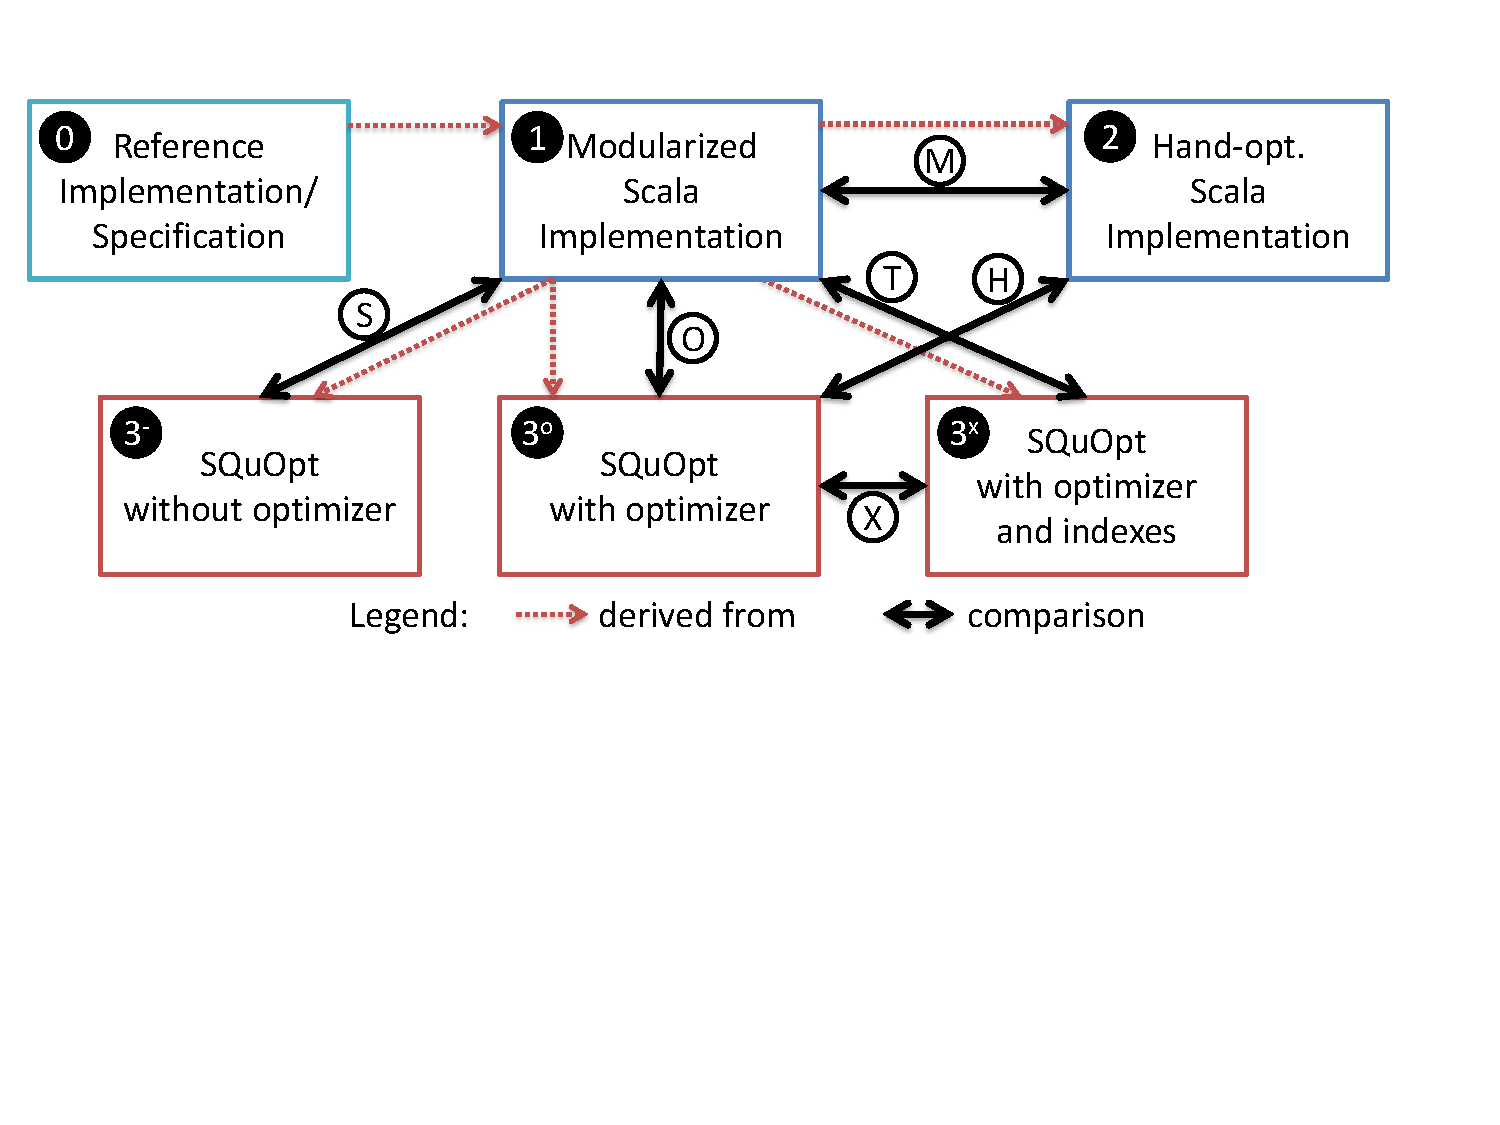
\includegraphics[width=\linewidth]{aosd13/graphs/measurements-overview}
	\caption{Measurement Setup: Overview}
	\label{fig:measurements-overview}
\end{figure}


\subsection{Experimental Units}




%selecting queries
%\begin{table*}
%\begin{tabular}{ll}\toprule
%Identifier & Description \\ \midrule
%PROTECTED\_FIELD % Findbugs: CI\_CONFUSED\_INHERITANCE
%%	& % Idealized: 4
%	& Class is final but declares protected field \\
%NO\_CLONE % Findbugs: CN\_IDOM
%%	& % Idealized: 9
%	&  Class implements Cloneable but does not define or use clone method \\
%SUPER\_CLONE\_MISSING % Findbugs: CN\_IDIOM\_NO\_SUPER\_CALL
%%	& % Idealized: 11
%	& The clone method does not call super.clone() \\
%NOT\_CLONEABLE % Findbugs: CN\_IMPLEMENTS\_CLONE\_BUT\_NOT\_CLONEABLE
%%	& % Idealized: 5
%	& Class defines clone() but doesn't implement Cloneable\\
%COVARIANT\_COMPARETO % Findbugs CO\_ABSTRACT\_SELF \& CO\_SELF\_NO\_OBJECT
%%	& % Idealized: 7
%	& Covariant compareTo() method defined\\
%GC\_CALL % Findbugs:  DM\_GC
%%	& % Idealized: 12
%	& Explicit garbage collection; extremely dubious except in benchmarking code\\
%RUN\_FINALIZERS\_ON\_EXIT % Findbugs DM\_RUN\_FINALIZERS\_ON\_EXIT
%%	& % Idealized: 12
%	& Method invokes dangerous method runFinalizersOnExit\\
%COVARIANT\_EQUALS %Findbugs: EQ\_ABSTRACT\_SELF
%%	& % Idealized: 4
%	& Abstract class defines covariant equals() method \\
%FINALIZER\_NOT\_PROTECTED % Findbugs: FI_PUBLIC_SHOULD_BE_PROTECTED
%%	& % Idealized: 6
%	& Finalizer should be protected, not public\\
%%NO\_SUITABLE\_CONSTRUCTOR% Findbugs: SE\_NO\_SUITABLE\_CONSTRUCTOR
%%	& % Idealized: 7
%%	& Class is Serializable but its superclass doesn't define a void constructor\\
%UNUSED\_PRIVATE\_FIELD % Findbugs: UUF\_UNUSED\_FIELD
%%	& % Idealized: 23
%	& The value of a private field is not read\\
%DONT\_CATCH\_IMSE  %Findbugs: IMSE\_DONT\_CATCH\_IMSE
%%	& % Idealized: 5
%	& Dubious catching of IllegalMonitorStateException \\\bottomrule
%\end{tabular}
%\nocaptionrule\caption{Implemented Analyses}
%\label{table:implemented-analyses}
%\end{table*}


\newcommand{\captionEvalTable}{%
As in in \cref{sec:implemenationsandspeedups}, (1) denotes the modular Scala
implementation, (2) the hand-optimized Scala one, and ($3^-$), ($3^o$), ($3^x$)
refer to the {\LoS} implementation when run, respectively, without
optimizations, with optimizations, with optimizations and indexing.
Queries marked with the $R$ superscript were selected by random sampling.}
\newcommand{\tablerowsize}{\scriptsize}
\begin{sidewaystable}[ph!]
\centering
\input{\graphPath{EvalTable}}
\nocaptionrule\caption{Performance results. \captionEvalTable}
\label{table:performance}
\end{sidewaystable}



\begin{table}[h]
  \centering
  \footnotesize
\input{\graphPath{EvalSummaryTable}}
\nocaptionrule\caption{Average performance ratios.
This table summarizes all interesting performance ratios across all queries,
using the geometric mean~\citep{Fleming86}.
The meaning of speedups is discussed in \cref{sec:implemenationsandspeedups}.}
\label{table:performanceAvg}
\end{table}

\begin{table}[h!]
\begin{tabular}{p{7cm}r}\toprule
Abstraction & Used \\ \midrule
% calculate class hierarchy & 5 \\
All fields in all class files	& 4\\
All methods in all class files	& 3\\
All method bodies in all class files	& 3\\
All instructions in all method bodies and their bytecode index	& 5\\
Sliding window (size $n$) over all instructions (and their index) &	3\\
\bottomrule
\end{tabular}\\
\nocaptionrule\caption{Description of abstractions removed during hand-optimization and number of queries where the abstraction is used (and optimized away).}
\label{table:implemented-abstractions}
\end{table}

\begin{extraEval}
\begin{table*}[tb]
\centering
\begin{tabular}{l*{3}{r@{}c@{}l}r*{2}{r@{}c@{}l}}\toprule
Name&\multicolumn{3}{c}{Base impl.\ (in ms)}&\multicolumn{3}{c}{Modular impl}&\multicolumn{3}{c}{Optimiz.\ time}&IS&\multicolumn{3}{c}{OS}&\multicolumn{3}{c}{OS-Opt}\\\midrule
\input{\graphPath{table}}
\bottomrule
\end{tabular}
\nocaptionrule\caption{Old performance results table}
\label{table:performanceOld}
\end{table*}
\end{extraEval}


As experimental units, we sampled a set of queries on code structures from FindBugs 2.0~\citep{DBLP:journals/sigplan/HovemeyerP04}. FindBugs is a popular bug-finding tool for Java Bytecode available as open source. To detect instances of bug patterns, it queries a structural in-memory representation of a code base (extracted from bytecode).
Concretely, a single loop traverses each class and invokes all visitors (implemented as listeners) on each element of the class. Many visitors, in turn, perform activities concerning multiple bug detectors which are fused together. An extreme example is that, in FindBugs, query \queryRUNFINALIZERSONEXIT{} is defined in class \code{DumbMethods} together with other 41 bug detectors for distinct types of bugs.
Typically a bug detector is furthermore scattered across the different methods of the visitor, which handle different elements of the class.
We believe this architecture has been chosen to achieve good performance; however, we do not consider such manual fusion of distinct bug detectors together as modular. We selected queries from FindBugs because they represent typical non-trivial queries on in-memory collections and because we believe our framework allows expressing them more modularly.

We sampled queries in two batches. First, we manually selected \manualQueryCount~queries (from approx.\ 400~queries in FindBugs), chosen mainly to evaluate the potential speedups of indexing (queries that primarily looked for declarations of classes, methods, or fields with specific properties, queries that inspect the type hierarchy, and queries that required analyzing methods implementation).
Subsequently, we \emph{randomly} selected a batch of \randomQueryCount~additional queries. 
The batch excluded queries that rely on control-/dataflow analyses (i.e., analyzing the effect of bytecode instructions on the stack), due to limitations of the bytecode tookit we use.
In total, we have \queryCount{} queries as listed in Table~\ref{table:performance} (the randomly selected queries are marked with the superscript $R$).




%Omit - this only showcases BAT, not our code. Show our implementation instead.
\begin{figure}
\centering
%\begin{lstlisting}
%for {
%  cf <- classFiles
%  m @ Method(_, "equals", MethodDescriptor(Seq(cf.thisClass), BooleanType), _) <- cf.methods 
%  if m.isAbstract
%} yield (cf, m)
%\end{lstlisting}
%import BATLifting._
\begin{lstlisting}
for {
  classFile <- classFiles.asSquopt
  method <- classFile.methods
  if method.isAbstract && method.name ==# "equals" && method.descriptor.returnType ==# BooleanType
  parameterTypes <- Let(method.descriptor.parameterTypes)
  if parameterTypes.length ==# 1 && parameterTypes(0) ==# classFile.thisClass
} yield (classFile, method)
\end{lstlisting}
\caption{Find covariant \code{equals} methods.}
\label{fig:covariant-equals}
\end{figure}



%reimplementation
We implemented each query three times (see implementations (1)--(3) in Sec.~\ref{sec:implemenationsandspeedups}) following the specifications given in the FindBugs documentation (0). Instead of using a hierarchy of visitors as the original implementations of the queries in FindBugs, we wrote the queries as for-comprehensions in Scala on an in-memory representation created by the Scala toolkit BAT\@.\footnote{\url{http://github.com/Delors/BAT}}
BAT in particular provides comprehensive support for 
writing queries against Java bytecode in an idiomatic way.
We exemplify an analysis in Fig.~\ref{fig:covariant-equals}: It detects all co-variant \code{equals} methods in a project by iterating over all class files (line 2) and all methods, searching for methods named ``\code{equals}'' that return a boolean value and define a single parameter of the type of the current class. 


\smartParagraph{Abstractions}
In the reference implementations (1), we identified several reusable abstractions as shown in Table~\ref{table:implemented-abstractions}. 
The reference implementations of all queries except \querySEBADFIELDINNERCLASS{} use exactly one of these abstractions, which encapsulate the main loops of the queries.

\smartParagraph{Indexes}
For executing ($3^x$) (\LoS\ with indexes), we have constructed three indexes to speed up navigation over the queried data of queries 1--\manualQueryCount{}: Indexes for method name, exception handlers, and instruction types. We illustrate the implementation of the method-name index in Fig.~\ref{fig:indexes}: it produces a collection of all methods and then indexes them using \code{indexBy}; its argument extracts from an entry the key, that is the method name.
We selected which indexes to implement using guidance from \LoS{} itself; during optimizations, \LoS{} reports which indexes it could have applied to the given query. Among those, we tried to select indexes giving a reasonable compromise between construction cost and optimization speedup.
%% If we want to show the raw data, we could use this LaTeX code - but we need updated, and correct, data!
We first measured the construction cost of these indexes:

\begin{center}
\begin{tabular}{l*{1}{r@{}c@{}l}}\toprule
Index&\multicolumn{3}{c}{Elapsed time (ms)}\\\midrule

Method name&$97.99$&$\pm$&$2.94$\\
Exception handlers&$179.29$&$\pm$&$3.21$\\
Instruction type&$4166.49$&$\pm$&$202.85$\\

\bottomrule
\end{tabular}
\end{center}
For our test data, index construction takes less than 200 ms for the first two indexes, which is moderate compared to the time for loading the bytecode in the BAT representation ($\readingClassFilesTime$). Building the instruction index took around 4 seconds, which we consider acceptable since this index maps each type of instruction (e.g.\ \code{INSTANCEOF}) to a collection of all bytecode instructions of that type.
%Valid question: why does the exception-handler index take so much more than the query it optimizes? That's because indexes are interpreted. But it's best not to say it. Also, we already discuss this later convincingly.

%The first index maps any method name to the corresponding methods (together with containing classes), and is used by many different queries. Its implementation is shown in Fig.~\ref{fig:indexes}: the code shown first produces a collection of all methods and then indexes them using \code{indexBy}; its argument extracts from an entry the key, that is the method name.
%The second index maps any exception type to exception handlers catching them (together with the containing method bodies, methods and class).
%The third index allows to look for occurrences of bytecode instructions of a given type; it maps any type of bytecode instruction (like \code{INVOKESTATIC}, \code{INVOKEVIRTUAL} and so on) to its occurrences.

\begin{figure}
\centering
\begin{lstlisting}
val methodNameIdx: Exp[Map[String, Seq[(ClassFile, Method)]]] = (for {
  classFile <- classFiles.asSquopt
  method <- classFile.methods
} yield (classFile, method)).indexBy(entry => entry._2.name)
\end{lstlisting}
\caption{A simple index definition}
\label{fig:indexes}
\end{figure}



\subsection{Measurement Setup}
To measure performance, we executed the queries on the preinstalled JDK class library (\texttt{rt.jar}), containing 58M of uncompressed Java bytecode.
We also performed a preliminary evaluation by running queries on the much smaller ScalaTest library, getting comparable results that we hence do not discuss.
Experiments were run on a 8-core Intel Core i7-2600, 3.40 GHz, with 8 GB of RAM, running Scientific Linux release 6.2.
The benchmark code itself is single-threaded, so it uses only one core; however the JVM used also other cores to offload garbage collection.
We used the preinstalled OpenJDK Java version 1.7.0\_05-icedtea and Scala 2.10.0-M7.

We measure steady-state performance as recommended by \citet{Georges07rigorousJavaPerformance}. We invoke the JVM $p = 15$ times;
at the beginning of each JVM invocation, all the bytecode to analyze is loaded in memory and converted into BAT's representation.
In each JVM invocation, we iterate each benchmark until the variations of results becomes low enough. We measure the variations of results through the coefficient of variation (CoV; standard deviation divided by the mean). Thus, we iterate each benchmark until the CoV in the last $k = \kZrememberedSampleLoops$ iterations drops under the threshold $\theta = \thetaZmaxCov$, or until we complete $q = \qZmaxLoops$ iterations.
We report the arithmetic mean of these measurements (and also report the usually low standard deviation on our web page).
%PG: I had p = 3, k = 50, theta = 0.02, q = 1000, but changed the parameters when running more queries.

\subsection{Results}

\smartParagraph{Correctness} We machine-checked that for each query, all variants in Table~\ref{table:performance} agree.

\smartParagraph{Modularization Overhead}
We first observe that performance suffers significantly when using the abstractions we described in Table~\ref{table:implemented-abstractions}. These abstractions, while natural in the domain and in the setting of a declarative language, are not idiomatic in Java or Scala because, without optimization, they
will obviously lead to bad performance. They are still useful abstractions from the point of view of modularity, though---as indicated by Table \ref{table:implemented-abstractions}---and as such it would be desirable if one could use them without paying the performance penalty.


\smartParagraph{Scala Implementations vs.\ FindBugs}
Before actually comparing between the different Scala and \LoS\ implementations, we first ensured that the implementations are comparable to the original FindBugs implementation. A direct comparison between the FindBugs reference implementation and any of our implementations is not possible in a rigorous and fair manner. FindBugs bug detectors are not fully modularized, therefore we cannot reasonably isolate the implementation of the selected queries from support code. Furthermore, the architecture of the implementation has many differences that affect performance: among others, FindBugs also uses multithreading. Moreover, while in our case each query loops over all classes, in FindBugs, as discussed above, a single loop considers each class and invokes all visitors (implemented as listeners) on it.

We measured \emph{startup performance}~\citep{Georges07rigorousJavaPerformance}, that is the performance of running the queries only once, to minimize the effect of compiler optimizations.
We setup our \LoS-based analyses to only perform optimization and run the optimized query. To setup FindBugs, we manually disabled all unrelated bug detectors; we also made the modified FindBugs source code available. The result is that the performance of the Scala implementations of the queries ($3^-$) has performance of the same order of magnitude as the original FindBugs queries -- in our tests, the \LoS\ implementation was about twice as fast. However, since the comparison cannot be made fair, we refrained from a more detailed investigation.

% XXX HACK
\smartParagraph{SQuOpt Overhead and Optimization Potential}
We present the results of our benchmarks in Table~\ref{table:performance}.
Column names refer to a few of the definitions described above; for readability, we do not present all the ratios previously introduced for each query, but report the raw data.
In Table~\ref{table:performanceAvg}, we report the geometric mean \cite{Fleming86} of each ratio, computed with the same weight for each query.

%queries are between \maxInterpOver{}x slower and \maxInvInterpOver{}x faster; on average \LoS\ queries are \geoMeanInvInterpOver{}x faster.
%\minInvInterpOver{}x and \maxInvInterpOver{}x---that is, queries are between \minInterpOver{}x and
We see that, in its current implementation, \LoS\ can cause a overhead S
(1/$3^-$) up to \maxInterpOver{}x. On average \LoS\ queries are
\geoMeanInterpOver{}x faster. These differences are due to minor implementation
details of certain collection operators.
For query $18^R$, instead, we have that the the basic \LoS\ implementation is \maxInvInterpOver{}x faster and are investigating the reason; we suspect this might be related to the use of pattern matching in the original query.

As expected, not all queries benefit from optimizations;
out of \queryCount{} queries, optimization affords for \nSpeededUpQueries{} of them significant speedups ranging from a \minOptimSpeedup{} factor to a \maxOptimSpeedup{} factor; \nBigSpeededUpQueries{} queries are faster by a factor of at least \speedupBigThreshold{}.
Only queries \queryMSPKGPROTECT{}, \querySICINNERSHOULDBESTATICANON{} and \queryITAINEFFICIENTTOARRAY{} fail to recover any modularization overhead.

We have analyzed the behavior of a few queries after optimization, to understand why their performance has 
(or has not) improved.

Optimization makes query \querySEBADFIELDINNERCLASS{} slower; we believe this is because optimization replaces filtering by lazy filtering, which is usually faster, but not here.
Among queries where indexing succeeds, query \queryGCCALL{} has the least speedup. After optimization, this query uses the instruction-type index to find all occurrences of invocation opcodes (\code{INVOKESTATIC} and \code{INVOKEVIRTUAL}); after this step the query looks, among those invocations, for ones targeting \code{runFinalizersOnExit}. Since invocation opcodes are quite frequent, the used index is not very specific, hence it allows for little speedup (\speedupTGCCALL). However no other index applies to this query; moreover, our framework does not maintain any selectivity statistics on indexes to predict these effects.
Query \queryFIUSELESS{} benefits from indexing without any specific tuning on our part, because it looks for implementations of \code{finalize} with some characteristic, hence the highly selective method-name index applies.
After optimization, query \queryDONTCATCHIMSE{} becomes simply an index lookup on the index for exception handlers, looking for handlers of \code{IllegalMonitorStateException}; it is thus not surprising that its speedup is thus extremely high (\maxOptimSpeedup{}). This speedup relies on an index which is specific for this kind of query, and building this index is slower than executing the unoptimized query. On the other hand, building this index is entirely appropriate in a situation where similar queries are common enough. Similar considerations apply to usage of indexing in general, similarly to what happens in databases.

\smartParagraph{Optimization Overhead}
The current implementation of the optimizer is not yet optimized for speed (of the optimization algorithm). For instance, expression trees are traversed and rebuilt completely once for each transformation.
However, the optimization overhead is usually not excessive and 
is $\avgOptimTime \pm \stdDevOptimTime$ ms, varying between \minOptimTime{} ms and \maxOptimTime{} ms (mostly depending on the query size).

\smartParagraph{Limitations}
Although many speedups are encouraging, our optimizer is currently a proof-of-concept and we experienced some limitations:
\begin{itemize}
\item In a few cases hand-optimized queries are still faster than what the optimizer can produce. We believe these problems could be addressed by adding further optimizations.
\item Our implementation of indexing is currently limited to immutable collections. For mutable collections, indexes must be maintained incrementally. 
Since indexes are defined as special queries in {\LoS},  incremental index maintenance becomes an instance of incremental maintenance of query results, that is, of incremental view maintenance. We plan to support incremental view maintenance as part of future work; however,
indexing in the current form is already useful, as illustrated by our experimental results.
\end{itemize}

\smartParagraph{Threats to Validity}
With rigorous performance measurements and the chosen setup, our study was setup to maximize internal and construct validity. Although we did not involve an external domain expert and we did not compare the results of our queries with the ones from FindBugs (except while developing the queries), we believe that the queries adequately represent the modularity and performance characteristics of FindBugs and {\LoS}. However, since we selected only queries from a single project, external validity is limited. 
While we cannot generalize our results beyond FindBugs yet, we believe that the FindBugs queries are representative for complex in-memory queries performed by applications.


\smartParagraph{Summary}
We demonstrated on our real-world queries that relying on declarative abstractions in collection queries often causes a significant slowdown. As we have seen, using \LoS\ without optimization, or when no optimizations are possible, usually provides performance comparable to using standard Scala; however, \LoS\ optimizations can in most cases remove the slowdown due to declarative abstractions. Furthermore, relying on indexing allows to achieve even greater speedups while still using a declarative programming style.
Some implementation limitations restrict the effectiveness of our optimizer, but since this is a preliminary implementation, we believe our evaluation shows the great potential of optimizing queries to in-memory collections.


% vim: set tw=0:
